\documentclass[compress]{beamer}
\usepackage[utf8]{inputenc}
\usepackage[english]{babel}
\usepackage{hyperref}
\usepackage{ccicons}

\usepackage{tikz}
\usetikzlibrary{graphs, quotes, arrows.meta, matrix}

\newcommand\scalemath[2]{\scalebox{#1}{\mbox{\ensuremath{\displaystyle #2}}}}

\usetheme{default}
\usecolortheme{Nord}
\setbeamertemplate{navigation symbols}{}

\title{Teoria dei grafi}
\subtitle{DP su alberi e DAG}
\author{Lorenzo Ferrari, Davide Bartoli}
\date{\today}

\begin{document}

\begin{frame}
  \maketitle
\end{frame}

\begin{frame}{Table of contents}
  \tableofcontents
\end{frame}

\section{Parallelismo tra DP e DAG}
\subsection{DP e DAG}
\begin{frame}{Parallelismo tra DP e DAG}
    Nelle lezioni precedenti abbiamo detto che ``tutto \`e grafo'', troviamo grafi anche dove non ce li aspetteremmo.
    \pause
    \vfill
    Consideriamo una generica dp
    \begin{itemize}
        \item vediamo ogni stato come un nodo
        \item se lo stato $b$ dipende dallo stato $a$, rappresentiamo questa dipendenza con un arco orientato $(a, b)$
        \item per calcolare la dp, visitiamo i nodi in \textbf{ordinamento topologico}
    \end{itemize}
\end{frame}

\begin{frame}{Parallelismo tra DP e DAG}{Ordinamento topologico}
    \begin{block}{Ordinamento topologico}
        Per \textbf{ordinamento topologico} (in inglese \textit{topological sort} o \textit{toposort}), si intende un ordinamento dei nodi di un grafo diretto in modo che ogni nodo viene prima di tutti i nodi collegati ai suoi archi uscenti.
    \end{block}
    \pause
    Un grafo \`e un DAG \textbf{se e solo se} esiste un suo ordinamento topologico.
    \vfill
    \pause
    A seconda delle implementazioni della nostra dp, potrebbe essere necessario trovare un toposort\footnote{generalmente ne esistono pi\`u di uno}.
    \pause
    \vfill
    Se sappiamo il grafo \`e un dag, si pu\`o facilmente trovare un toposort con una dfs.


\end{frame}

\begin{frame}{Parallelismo tra DP e DAG}{Fibonacci}
    Prendiamo per esempio la dp dei numeri di Fibonacci
    \[
        F_n =
        \begin{cases}
            1 \quad & \text{per } 0 \leq n \leq 1 \\
            F_{n-1} + F_{n-2} & \text{per } n \geq 2
        \end{cases}
    \]
    \pause
    Il DAG equivalente \`e il seguente
    \begin{center}
        \scalebox{0.7}{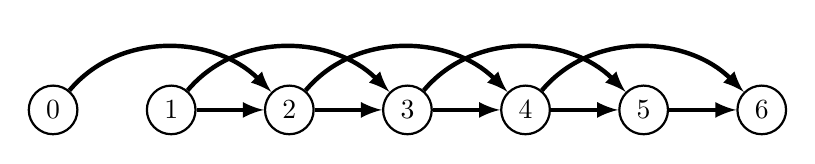
\begin{tikzpicture}
  \tikzset{vertex/.style = {draw, circle, thick}}
  \tikzset{arc/.style = {-latex, ultra thick}}
  % Nodes
  \node[vertex] (0) at (0, 0) {0};
  \node[vertex] (1) at (1.5, 0) {1};
  \node[vertex] (2) at (3, 0) {2};
  \node[vertex] (3) at (4.5, 0) {3};
  \node[vertex] (4) at (6, 0) {4};
  \node[vertex] (5) at (7.5, 0) {5};
  \node[vertex] (6) at (9, 0) {6};
  % Edges
  \draw[arc] (0) to[out=50] (2);
  \draw[arc] (1) edge (2);
  \draw[arc] (1) to[out=50] (3);
  \draw[arc] (2) edge (3);
  \draw[arc] (2) to[out=50] (4);
  \draw[arc] (3) edge (4);
  \draw[arc] (3) to[out=50] (5);
  \draw[arc] (4) edge (5);
  \draw[arc] (4) to[out=50] (6);
  \draw[arc] (5) edge (6);
\end{tikzpicture}
}
    \end{center}
\end{frame}

\begin{frame}{Parallelismo tra DP e DAG}
    Se ogni dp \`e un DAG, allora fare una dp su un DAG \`e molto pi\`u naturale di quel che sembra.
    \vfill
    Semplicemente le relazioni di dipendenza tra stati sono arbitrarie e vengono date in input.
    \vfill
    \begin{exampleblock}{Esempio}
        Dato un DAG, contare i percorsi da $0$ a $n-1$
    \end{exampleblock}
\end{frame}


\begin{frame}{Contare percorsi}{Implementazione}
    \makebox[\textwidth]{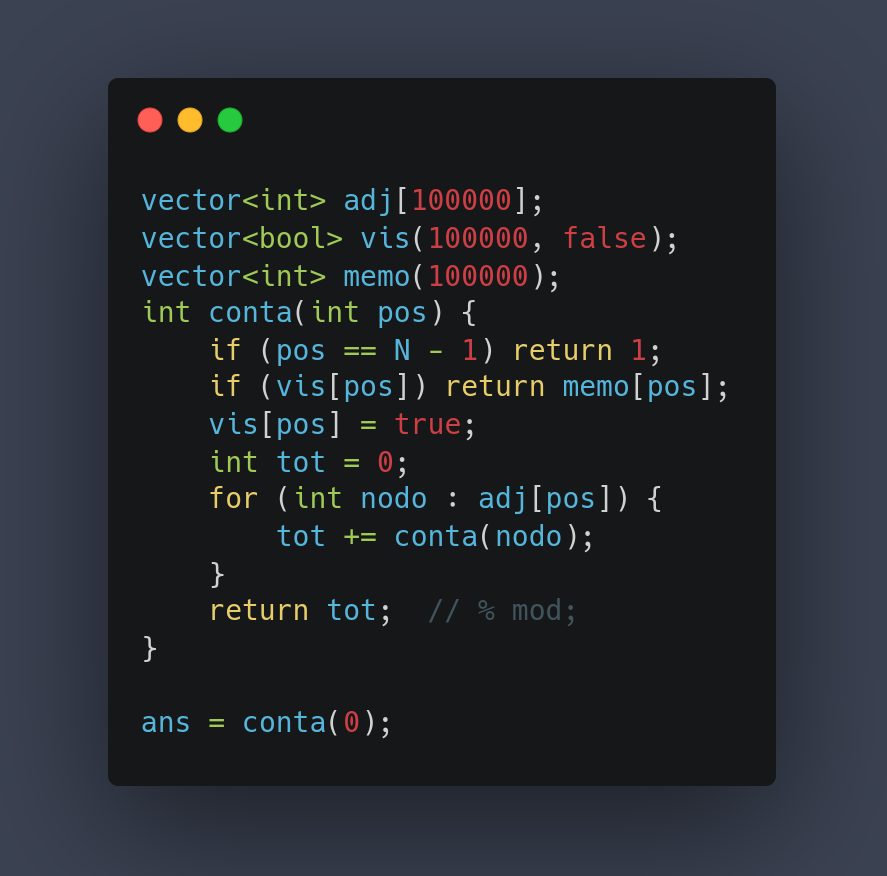
\includegraphics[scale=.28]{./img/count_path.png}}
\end{frame}

\subsection{DP e albero}
\begin{frame}{DP su albero}
    Possiamo applicare questa idea anche a problemi su alberi.\\
    \vfill
    \pause
    Nonostante gli alberi generalmente non siano DAG (dato che gli archi sono bidirezionali), possiamo sempre trovare un DAG equivalente,
    fissando un nodo radice e orientando gli archi verso i figli.\\
    \vfill
    \pause
    Questa idea ci permette di risolvere facilmente problemi su alberi, come ad esempio calcolare la dimensione di ogni sottoalbero.
\end{frame}

\section{Problemi}
\subsection{Problemi}
\begin{frame}{Problemi}
    \underline{\url{https://cses.fi/problemset/task/1674}}
    \underline{\url{https://cses.fi/problemset/task/1130}}
    \underline{\url{https://cses.fi/problemset/task/1131}}
    \underline{\url{https://training.olinfo.it/\#/task/traffic/statement}}
    \underline{\url{https://training.olinfo.it/\#/task/ois_magicforest/statement}}
    \underline{\url{https://training.olinfo.it/\#/task/ois_xmastree/statement}}
    \underline{\url{https://training.olinfo.it/\#/task/ois_picarats/statement}}
    \underline{\url{https://training.olinfo.it/\#/task/preoii_catene/statement}}
\end{frame}

\begin{frame}
    \begin{block}{}
        \begin{center}
        Fateci sapere come stanno andando le lezioni \\
        \underline{\url{https://forms.gle/WGPqv2ctQ34b4tz9A}}
        \end{center}
    \end{block}
\end{frame}

\end{document}
